\documentclass[aps,prx,reprint,superscriptaddress,nofootinbib,floatfix]{revtex4-2}

\usepackage[T1]{fontenc}
\usepackage[sc]{mathpazo}
\usepackage{amsmath,amssymb,amsthm}
\usepackage{bm}
\usepackage{tikz}
\usetikzlibrary{arrows.meta,decorations.pathreplacing,patterns}
\usepackage{xcolor}
\usepackage[colorlinks=true,linkcolor=blue!50!black,citecolor=blue!50!black,urlcolor=blue!50!black]{hyperref}

\newtheorem{definition}{Definition}
\newtheorem{lemma}{Lemma}
\newtheorem{theorem}{Theorem}
\newtheorem{proposition}{Proposition}
\theoremstyle{remark}
\newtheorem*{remark}{Remark}

% Notation
\newcommand{\Live}{L}                     % live facts
\newcommand{\justifies}{\Vdash}           % J \justifies_v alpha
\newcommand{\Rd}{\mathrm{Rd}}             % readers at a revision
\newcommand{\cut}{v}                      % cut of an action
\newcommand{\roster}{M}
\newcommand{\rec}{\mathcal R}             % the ledger's roster record
\newcommand{\derives}{\vdash}
\newcommand{\Adv}{\mathrm{Adv}}
\newcommand{\open}{\textsf{open}}
\newcommand{\closed}{\textsf{closed}}
\newcommand{\Static}{\mathrm{Scope}}
\newcommand{\cell}[2]{\parbox[t]{#1}{\raggedright #2\strut}}

\begin{document}

\title{Two clocks, one cut:\\ may--can concordance and revocation in MLS groups}

\author{Daniel Sobral}
\affiliation{Quside Technologies, Barcelona, Spain}

\date{25 October 2026}

\begin{abstract}
An authorization service decides who \emph{may} read or act in a group. A group-key protocol such as MLS decides who \emph{can}. The two descriptions run on different clocks, and a party removed from the first may keep the keys of the second. We give a minimal model in which both evolve, and we fix the event that makes the two clocks comparable: the \emph{cut}, the ledger revision at which an action is released. A protocol is in \emph{may--can concordance} when whoever can exercise a capability on an action may do so at that action's cut. A no-go result shows that oblivious composition of a correct authorization service with a correct group protocol is generically discordant. We give a construction made of four local rules (a fence, a removal commit, a release rule and an acceptance rule). We prove that it is concordant for reading and for acting, including delegated and invoked authority with cascading revocation. Read concordance factorizes into two parts. The first is a combinatorial statement about rosters, proved here by induction over the protocol's transitions. The second is a cryptographic property of MLS, key confinement: an epoch key is hidden from every party outside that epoch's roster. We derive key confinement from published theorems. The symbolic form is a corollary of the machine-checked analysis of TreeKEM. The computational form follows from the ETK theorem for RFC~9420, because every commit the construction issues is an operation ETK models. Write concordance reduces to signature unforgeability. We also searched every reachable state of a finite model, $1.56\times10^6$ states, against an adversary that never forgets a key. The search finds no violation, and deleting any one of nine rules or conditions produces a counterexample that the search finds unaided. A second no-go result states the price: the authorization ledger must be reachable at every release.
\end{abstract}

\maketitle

%=====================================================================
\section{Introduction}
%=====================================================================

Consider a group with three members, Alice, Bob and Carol, who share an end-to-end encrypted channel. An external authority, the \emph{ledger}, records who may read. At some instant the ledger revokes Alice. The ledger is correct: every later query returns ``Alice may not read.'' The group protocol is also correct. Alice is still in the current epoch and holds its key, because nobody has yet committed her removal. If Bob now sends a fresh message in the old epoch, Alice reads it. Neither component failed. Their composition did.

The difficulty is not a bug in either component but a mismatch of descriptions. The ledger describes authorization as a function of its revision number $v$. The group describes capability as a function of its epoch $e$. Nothing ties the two clocks together, so the phrase ``after Alice was revoked'' has no meaning for Bob's message until we say \emph{which event} defines ``now'' for that message. The situation resembles simultaneity in relativity: before one can compare two clocks, one must fix the event that serves as a common reference. Here that event is the moment the ledger \emph{releases} the action. We call the ledger revision at that moment the action's \emph{cut}.

With the cut fixed, the requirement is easy to state. Every party that \emph{can} exercise a capability on an action must have been one that \emph{may}, at the action's cut. When the two descriptions agree in this sense we say they are in \emph{may--can concordance}, or simply that the protocol is \emph{concordant}. When they disagree it is \emph{discordant}. Figure~\ref{fig:clocks} shows the \emph{discordance window} that opens when the release ignores the roster.

\begin{figure}[t]
\centering
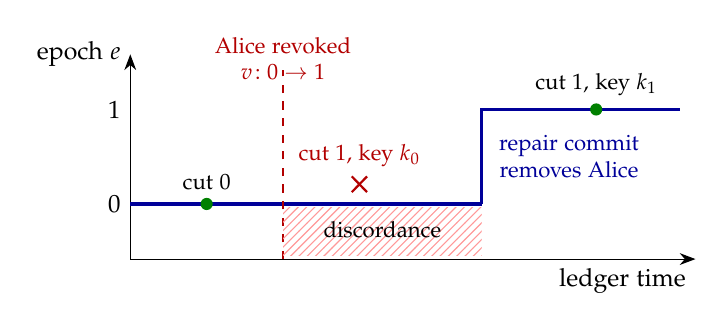
\begin{tikzpicture}[x=0.97cm,y=1.0cm,>={Stealth[length=2mm]}]
  % axes
  \draw[->] (0,0) -- (7.4,0) node[below left] {\small ledger time};
  \draw[->] (0,0) -- (0,2.6) node[left] {\small epoch $e$};
  \foreach \e in {0,1} \node[left] at (0,0.7+1.2*\e) {\small $\e$};
  % epoch staircase
  \draw[very thick,blue!60!black] (0,0.7) -- (4.6,0.7);
  \draw[very thick,blue!60!black] (4.6,0.7) -- (4.6,1.9) -- (7.2,1.9);
  % revocation
  \draw[dashed,red!70!black,thick] (2.0,0) -- (2.0,2.4);
  \node[red!70!black,align=center,font=\footnotesize] at (2.0,2.55) {Alice revoked\\ $v\!:0\to1$};
  % repair
  \node[blue!60!black,align=center,font=\footnotesize,anchor=west] at (4.7,1.3) {repair commit\\ removes Alice};
  % window
  \fill[pattern=north east lines,pattern color=red!40] (2.0,0.05) rectangle (4.6,0.65);
  \node[font=\footnotesize,align=center] at (3.3,0.38) {discordance};
  % releases
  \fill[green!50!black] (1.0,0.7) circle (2.2pt);
  \node[font=\footnotesize,above] at (1.0,0.75) {cut $0$};
  \draw[red!70!black,thick] (3.0,0.95) ++(-0.1,-0.1) -- ++(0.2,0.2) ++(-0.2,0) -- ++(0.2,-0.2);
  \node[font=\footnotesize,above,red!70!black] at (3.0,1.05) {cut $1$, key $k_0$};
  \fill[green!50!black] (6.1,1.9) circle (2.2pt);
  \node[font=\footnotesize,above] at (6.1,1.95) {cut $1$, key $k_1$};
\end{tikzpicture}
\caption{Two clocks. Horizontal: the ledger's history. Vertical: the group's epoch. Alice is revoked at revision 1, but she leaves the group only at the next epoch. A message released inside the hatched discordance window has cut 1 (Alice may not read) yet is protected under $k_0$, which Alice holds (she can). Messages released before the revocation (left dot) or after the repair (right dot) are concordant. The construction of Sec.~\ref{sec:construction} closes a \emph{fence} over the window, so no release happens there.}
\label{fig:clocks}
\end{figure}

\paragraph*{Results.} We work in a model that keeps only what the argument needs: a ledger of facts with lifetimes, justifications built from facts, and a group whose epochs have rosters and keys (Sec.~\ref{sec:model}). In this model:
\begin{enumerate}
\item Concordance is defined for reading and for acting [Eqs.~\eqref{eq:readconc} and \eqref{eq:writeconc}]. A no-go result shows that oblivious composition violates it (Proposition~\ref{prop:oblivious}).
\item Four local rules suffice for concordance (Sec.~\ref{sec:construction}). The proof of read concordance \emph{factorizes} into two parts. The first is a combinatorial lemma about rosters, roster inclusion (Lemma~\ref{lem:roster}), proved by induction. The second is one property of MLS, key confinement: an epoch key is hidden from every party outside that epoch's roster. The factorization theorem (Theorem~\ref{thm:read}) composes the two. Write concordance needs only signature unforgeability (Theorem~\ref{thm:write}).
\item Key confinement follows from published results under five conditions K1--K5, all enforced by the construction (Sec.~\ref{sec:K}). Symbolically, it is a corollary of the machine-checked TreeKEM theorem (Proposition~\ref{prop:Ksym}). Computationally, it follows from the ETK theorem (Proposition~\ref{prop:Kcomp}). To make that possible, the policy binding lives in the ledger's signed acknowledgement of each commit, not in the MLS group context.
\item Delegated authority and invocations need no new theory. A delegation chain is a justification with more facts, and cascading revocation follows from one locality property (Sec.~\ref{sec:delegation}).
\item The cost is a ledger contact per release, and a second no-go result shows that it cannot be avoided at the release cut (Proposition~\ref{prop:price}). Under stated assumptions the construction makes progress after a revocation (Proposition~\ref{prop:progress}).
\item An exhaustive finite-state search supports the claims (Sec.~\ref{sec:evidence}). Its adversary never forgets a key, and every rule is shown necessary by an automatically found counterexample.
\end{enumerate}
Key confinement is the only cryptographic property of MLS that we use. Appendix~\ref{app:mapping} matches it, case by case, against the exact statements of the two analyses it rests on.

%=====================================================================
\section{Model}\label{sec:model}
%=====================================================================

\paragraph*{The ledger.} The ledger is a totally ordered sequence of revisions $v=0,1,2,\dots$. Its content is a set of \emph{facts} $F$. A fact is a root grant, a delegation from one party to another, or an invocation that lets one party act for another. At revision $v$ a subset $\Live_v\subseteq F$ of facts is \emph{live}. A revocation removes a fact from the live set. Re-granting never revives a fact; it issues a new one with a new generation number. The lifetime of every fact is therefore an interval:
\begin{equation}
f\in \Live_u,\; f\in \Live_w,\; u<v<w \;\Longrightarrow\; f\in \Live_v .
\label{eq:interval}
\end{equation}

\paragraph*{Justifications.} An \emph{action type} $\alpha=(p,r,x)$ names a party $p$, a right $r\in\{\text{read},\text{write},\text{admin},\text{admit}\}$ and a resource or group $x$. A \emph{justification} is a finite set of facts $J\subseteq F$. We write $J\justifies_v\alpha$ when $J$ justifies $\alpha$ at revision $v$. The single structural property we require is that authorization depends on time only through liveness:
\begin{equation}
J\justifies_v\alpha \iff J\subseteq \Live_v \;\wedge\; \Static(J,\alpha),
\label{eq:locality}
\end{equation}
where the predicate $\Static$ does not depend on $v$. It checks everything about the \emph{content} of the facts: that a delegation chain is connected, that each link narrows the rights and resources of its parent, and that the chain ends at $p$ with right $r$ on $x$. Equation~\eqref{eq:locality} says that every change of authorization is a ledger event. A delegation that expires at a wall-clock time must be modeled as a revocation recorded on the ledger at that time.

The \emph{readers} of group $g$ at revision $v$ are
\begin{equation}
\Rd_v(g)=\{\,p:\exists J\;\; J\justifies_v (p,\text{read},g)\,\}.
\label{eq:readers}
\end{equation}

\paragraph*{The group.} The group moves through epochs $e=0,1,2,\dots$. Epoch $e$ has a roster $\roster_e$ of members (one entry per device incarnation) and an epoch key $k_e$, from which the message keys of that epoch are derived. A party \emph{holds} everything it has ever received. No party is ever assumed to forget. We write $S\derives k$ when the parties in set $S$, pooling everything they have ever held, can compute $k$.

\paragraph*{Actions and their cut.} A \emph{protected action} $a$ is a single read-protected message, a write, or a control operation (a proposal or commit, which is an admin or admit action). Every action passes through one atomic \emph{release} step at the ledger. The ledger revision read by that step is the action's cut,
\begin{equation}
\cut(a)=\text{revision at the release of }a .
\label{eq:cut}
\end{equation}
A read action is protected under the key of an epoch $e(a)$. Neither encryption, transmission nor receipt moves the cut. A message released before a revocation and read afterwards is judged at the earlier revision. This is a deliberate choice of semantics: the \emph{release cut}. Causal or lease-based cuts are possible and lead to different properties, which we do not treat.

%=====================================================================
\section{Concordance}\label{sec:concordance}
%=====================================================================

\begin{definition}[Read concordance]
A protocol is \emph{read-concordant} if, in every execution, for every released read action $a$ in group $g$,
\begin{equation}
\{p\}\derives k_{e(a)} \;\Longrightarrow\; p\in \Rd_{\cut(a)}(g).
\label{eq:readconc}
\end{equation}
\end{definition}
In words, nobody can derive the key of a message without having been a reader at that message's cut. Equation~\eqref{eq:readconc} is the symbolic statement. The computational statement is an indistinguishability game rather than an event. Fix a challenge action $a$ in group $g$. Let the \emph{coalition} $C_a=\{\,p:p\notin \Rd_{\cut(a)}(g)\,\}$ be all parties that were not readers at its cut. The adversary controls the network, receives everything the members of $C_a$ ever hold, at any time, and chooses two equal-length messages $m_0,m_1$. The honest sender protects $m_b$ for a uniform bit $b$. The protocol is read-concordant if no efficient adversary guesses $b$ with probability non-negligibly above $1/2$. We denote that excess by $\Adv^{\rm read}$.

Two things lie outside this definition, deliberately. A party that \emph{was} a reader at the cut may read the message at any later time and leak it; no protocol can prevent that. Plaintext obtained before a revocation is not erased.

\begin{definition}[Write concordance]
A protocol is \emph{write-concordant} if, whenever an honest receiver accepts an action $a$ of type $\alpha$,
\begin{equation}
\exists J:\; J\justifies_{\cut(a)}\alpha,\quad \text{bytes accepted}=\text{bytes released},
\label{eq:writeconc}
\end{equation}
and each receiver accepts each release at most once.
\end{definition}
Write concordance concerns events observed at honest receivers, so it is a property of executions directly. It applies equally to writes, to administrative commits (where the ``receiver'' is the sequencer and every member processing the commit) and to admissions.

\begin{proposition}[No-go for oblivious composition]\label{prop:oblivious}
Let the ledger be an ideal authorization service and the group an ideal group-key protocol, each meeting its own specification. Call the composition \emph{oblivious} if the release of an action does not depend on the group's roster. Every oblivious composition has an execution violating Eq.~\eqref{eq:readconc}.
\end{proposition}
\begin{proof}
Start with $\roster_0=\{A,B\}$, both readers at revision 0. The ledger revokes $A$'s read fact, moving to revision 1. Before any removal commit, $B$ releases a message $a$ in epoch 0, so $\cut(a)=1$ and $e(a)=0$. Since $A\in\roster_0$, the group protocol has given $A$ the key, so $\{A\}\derives k_0$. Yet $A\notin \Rd_1(g)$.
\end{proof}

The proof uses no broken cryptography, no crash and no replay. It sits in the discordance window of Fig.~\ref{fig:clocks}. Any concordant protocol must ensure that no read release ever falls in such a window.

%=====================================================================
\section{The construction}\label{sec:construction}
%=====================================================================

The ledger keeps, besides its facts, four pieces of state: a \emph{fence} $\varphi\in\{\open,\closed\}$ for each group; the canonical epoch $e^\ast$; a \emph{roster record} $\rec=\{(p,J_p)\}$, listing for each member the justification under which it was admitted; and a set of spent (action, receiver) pairs. Every ledger step is atomic. The construction consists of four rules.

\paragraph*{Rule F (fence).} In the same atomic step that changes the live set from $\Live_v$ to $\Live_{v+1}$, the ledger sets $\varphi\gets\closed$ if some recorded justification is no longer live:
\begin{equation}
\exists (p,J_p)\in\rec:\; J_p\not\subseteq \Live_{v+1}\;\Longrightarrow\;\varphi\gets\closed .
\label{eq:ruleF}
\end{equation}

\paragraph*{Rule C (commit).} While $\varphi=\closed$, a member $q$ whose own record is still live builds an MLS commit for epoch $e^\ast{+}1$. The commit removes \emph{exactly} the members whose records are dead and carries a fresh path secret (an UpdatePath). The ledger accepts the commit only if its parent is the current epoch, which is a compare-and-swap. It installs
\begin{equation}
\begin{aligned}
\rec&\gets\{(p,J_p)\in\rec: J_p\subseteq \Live_v\},\\
\roster_{e^\ast+1}&=\{p:(p,\cdot)\in\rec\},
\end{aligned}
\label{eq:ruleC}
\end{equation}
and opens the fence. Admission is the same step in reverse. With the fence open, a commit may add $p$ together with a $J_p$ that satisfies $J_p\justifies_v(p,\text{read},g)$. For each installed commit, the ledger signs an \emph{acknowledgement} binding the exact commit, the new epoch and the current revision $v$. A client merges a commit only if it holds that acknowledgement. Commits carry only Add and Remove proposals (or none) and the required path. No external commits, group-context changes, resumption pre-shared keys or re-initializations are accepted.

\paragraph*{Rule R (release).} The ledger releases a read action $a$ only if $\varphi=\open$ and the sender's epoch equals $e^\ast$. It releases a write or control action of type $\alpha$ only if the presented justification satisfies $J\justifies_v\alpha$. In each case it signs a certificate binding the action identifier, a hash of the frozen content, the cut $v$, the epoch, and $J$ or $\rec$. The sender then protects the content once, with the hash of the certificate as MLS associated data.

\paragraph*{Rule A (accept).} An honest receiver accepts an action only if the certificate verifies and binds the exact bytes received, and only after the ledger has atomically marked the pair (action, receiver) as spent.

Rules F and C govern \emph{who holds keys}, and Rules R and A govern \emph{what is released and accepted}. The roster record makes the ledger deliberately pessimistic. A member whose recorded justification died is removed, even if some other justification would still cover it. That costs availability, never safety.

%=====================================================================
\section{Results}\label{sec:results}
%=====================================================================

\subsection{The fence lemma}

\begin{lemma}[Fence]\label{lem:fence}
In every reachable state of the ledger,
\begin{equation}
\varphi=\open \;\Longrightarrow\; \forall (p,J_p)\in\rec:\; J_p\subseteq\Live_v ,
\label{eq:fence}
\end{equation}
where $v$ is the current revision. Moreover the parties of $\rec$ are exactly $\roster_{e^\ast}$.
\end{lemma}
\begin{proof}
By induction over the ledger's steps. Initially every record was admitted with a live justification and $\varphi=\open$. A step of the ledger is one of the following.
\begin{enumerate}
\item A \emph{change of the live set} from $\Live_v$ to $\Live_{v+1}$ (a revocation or a new grant). If every record is still live, Eq.~\eqref{eq:fence} continues to hold. Otherwise Rule F closes the fence in the same step, and the implication holds vacuously.
\item A \emph{removal commit} (Rule C). It keeps exactly the live records and opens the fence, so Eq.~\eqref{eq:fence} holds by construction. The new roster equals the kept records by Eq.~\eqref{eq:ruleC}, and the compare-and-swap ensures that only one child of $e^\ast$ is installed.
\item An \emph{admission} (Rule C with the fence open). It adds one record whose justification satisfies $J_p\justifies_v(p,\text{read},g)$, hence $J_p\subseteq\Live_v$ by Eq.~\eqref{eq:locality}. The revision is unchanged.
\item A \emph{release, acceptance or spend} (Rules R and A). It changes none of $v$, $\Live_v$, $\rec$ or $\varphi$.
\end{enumerate}
Steps taken locally by clients (processing a commit, crashing, restoring an old snapshot) do not change ledger state. A client that has not installed $e^\ast$ cannot obtain a release, because Rule R compares its epoch with $e^\ast$.
\end{proof}

\begin{lemma}[Roster inclusion]\label{lem:roster}
For every released read action $a$ in group $g$,
\begin{equation}
\roster_{e(a)} \subseteq \Rd_{\cut(a)}(g).
\label{eq:roster}
\end{equation}
\end{lemma}
\begin{proof}
By Rule R, at the release $\varphi=\open$ and $e(a)=e^\ast$. Take $p\in\roster_{e(a)}$ with record $(p,J_p)$. Lemma~\ref{lem:fence} gives $J_p\subseteq\Live_{\cut(a)}$. When $p$ was admitted, $J_p\justifies(p,\text{read},g)$ held, so $\Static(J_p,(p,\text{read},g))$ holds, and $\Static$ does not depend on the revision. By Eq.~\eqref{eq:locality}, $J_p\justifies_{\cut(a)}(p,\text{read},g)$, that is, $p\in\Rd_{\cut(a)}(g)$.
\end{proof}

Lemma~\ref{lem:roster} is purely combinatorial. It mentions no key and no adversary. It says that the ledger never releases a read action into an epoch whose roster contains a non-reader. What remains is to connect rosters to keys.

\subsection{Key confinement}\label{sec:K}

Lemma~\ref{lem:roster} concerns rosters. To reach keys we need one property of MLS. Informally, an epoch key leaks only through a member of that epoch. We state it under five conditions, each enforced by the construction or by the choice of parameters.
\begin{enumerate}
\item[K1.] \emph{Conformance.} Every commit is processed as RFC~9420 prescribes, so a commit containing a Remove carries a fresh UpdatePath. Honest members draw good randomness.
\item[K2.] \emph{Member-only, modeled commits.} The ledger installs only commits sent by a current member. A commit carries Add or Remove proposals or none, a path where required, and possibly a new signature key for the committer. There are no external commits, no external self-add proposals, no group-context changes, and no re-initialization or branching.
\item[K3.] \emph{One road to message keys.} Message keys are derived from the epoch secret only through the key schedule and the secret tree. No exporter secret is used outside Rule R.
\item[K4.] \emph{Strong primitives.} Members and the ledger sign with a strongly unforgeable (SUF-CMA) scheme, and the public-key encryption of the suite is IND-CCA. Both suites of the implementation are discussed after Proposition~\ref{prop:Kcomp}.
\item[K5.] \emph{Fresh incarnations.} A party admitted or re-admitted enters with signature, initialization and leaf keys that no other incarnation ever used.
\end{enumerate}

\begin{proposition}[Key confinement, symbolic]\label{prop:Ksym}
Assume K1--K5, in the Dolev--Yao model. Let $e$ be an epoch on the canonical chain and $S$ a set of parties with $S\cap\roster_e=\emptyset$. An attacker that holds every state of every member of $S$, at every time, can derive neither the epoch secret $k_e$ nor any message key of epoch $e$:
\begin{equation}
S\cap\roster_e=\emptyset\;\Longrightarrow\; S\not\derives k_e .
\label{eq:Ksym}
\end{equation}
\end{proposition}
\begin{proof}
Let $p$ be an honest member of epoch $e$, for instance the sender of the message in question. Wallez, Protzenko and Bhargavan prove, in a machine-checked DY$^\ast$ development, a confidentiality theorem for TreeKEM from $p$'s point of view~\cite{treekem-fstar,wallez-thesis}. If the attacker knows the epoch secret $K_n$, then one of ten listed compromise cases holds. Appendix~\ref{app:mapping} gives the full list. The cases fall into three groups.
\begin{enumerate}
\item[(i)] Eight cases require that the attacker compromised a state belonging to a participant or joiner of epoch $n$, or to the inviter, who is a participant. The state may be an epoch secret, initialization key, signature key or node keys. By K5 the states of an incarnation are disjoint from those of every other incarnation, and $S\cap\roster_n=\emptyset$, so none of these states is ever compromised.
\item[(ii)] One case requires $K_{n-1}$ together with an add-only commit. Then $\roster_{n-1}\subseteq\roster_n$, so $S\cap\roster_{n-1}=\emptyset$, and induction on $n$ applies.
\item[(iii)] One case applies the theorem to the inviter's view of the same epoch and roster. The chain of inviters is finite and ends at the creator of the group, whose own case belongs to group (i).
\end{enumerate}
Several cases also require the attacker to know the pre-shared keys. Those conjuncts only add conditions. Hence the attacker does not know $k_e$. Message keys are derived from $k_e$ by key derivation functions. In the symbolic model a derived value is known only from its inputs or from a state that stores it. The states of members of $\roster_e$ are not compromised, and K3 excludes other derivations.
\end{proof}

The machine-checked theorem covers commits with any mix of add, remove and update proposals, blank nodes, unmerged leaves, add-only commits, Welcome messages and pre-shared keys. It covers neither external commits nor bad randomness, which is why K1 and K2 appear. The grouping into (i)--(iii) is the manual step that Ref.~\cite{wallez-thesis} itself uses to derive remove-security from its theorem.

\begin{proposition}[Key confinement, computational]\label{prop:Kcomp}
Assume K1--K5. By K2, every commit on the chain is an operation modeled by ETK~\cite{etk}. Admission is a commit with Add proposals, repair a commit with Remove proposals and a path, and rekey a commit with a path and a new signature key. Then every epoch $e$ with $S\cap\roster_e=\emptyset$ satisfies ETK's predicate $\mathsf{safe}$, even when $S$ is fully corrupted, randomness included. Consequently, by Theorem~1 of Ref.~\cite{etk}, the application secret of $e$ is indistinguishable from random, except with the advantage $\Adv^{\rm ETK}$ of distinguishing ETK from its ideal functionality $\mathcal F_{\rm ECGKA}$. That theorem assumes IND-CCA public-key encryption and SUF-CMA signatures, in the random-oracle model.
\end{proposition}
\begin{proof}
ETK's predicate declares an epoch unsafe if some member's secrets are exposed in it, or if one of five traversal clauses, a)--e), holds. Appendix~\ref{app:mapping} shows that none applies. Exposures are recorded only for members of the epoch, and none of them is in $S$. Clause a) needs an injected commit, which requires knowledge of the parent epoch. Clauses b) and c) need an added member whose signature key is exposed or who is corrupted later. By K5 and $S\cap\roster_e=\emptyset$, no such member exists. Clause d) needs some party's state at $e$ to be known. For members of $\roster_e$ this fails by K1 and K5. For a removed member, ETK's knowledge relation stops at the commit that removed it, whose \textsf{secrets-replaced} flag cuts the propagation. Clause e) concerns external commits, excluded by K2.
\end{proof}

\emph{Instantiating K4.} The implementation offers two MLS cipher suites. In the classical suite (\texttt{0x0001}) signatures are Ed25519 with strict verification, which is SUF-CMA~\cite{ed25519-provable}, and HPKE uses DHKEM over X25519, which is IND-CCA under the strong Diffie--Hellman assumption in the random-oracle model~\cite{dhies}. The default post-quantum suite (\texttt{0x0052}) uses ML-DSA-44 and X-Wing. FIPS~204 states SUF-CMA as a design goal of ML-DSA~\cite{fips204}. For Dilithium, on which ML-DSA is based, Ref.~\cite{kls18} bounds the SUF-CMA advantage in the quantum random-oracle model by MLWE, SelfTargetMSIS and MSIS. Reference~\cite{fsa-fix} later found and corrected a gap in the chosen-message step of that proof, for ordinary unforgeability only. A companion note~\cite{note-suf} writes out the strong case: the corrected reduction bounds a distinguishing advantage, so it applies to a strong-forgery predicate, and a forgery at a programmed oracle point gives two accepting transcripts with the same commitment and challenge, which reduces to MSIS. The note adds the message representative, deterministic signing and the encoding, and checks that both verifiers of the implementation reject non-canonical hints, as FIPS~204 requires. It holds in both random-oracle models and is not mechanized. X-Wing is IND-CCA if either X25519 (strong Diffie--Hellman, random-oracle model) or ML-KEM-768 is~\cite{xwing}. HPKE in base mode is a KEM--DEM composition, so it is IND-CCA when its KEM is IND-CCA and its AEAD is secure~\cite{cramer-shoup}. One limit remains. ETK's Theorem~1 is proved in the classical random-oracle model. With the post-quantum suite, Proposition~\ref{prop:Kcomp} therefore holds against classical adversaries. A second note~\cite{note-qrom} locates the only classical-only step of ETK's proof, three reductions that search the environment's oracle queries for a secret, and states the quantum version as a conjecture with five checks.

\emph{Where the policy binding lives.} An earlier design wrote the policy revision into the MLS group context through a GroupContextExtensions proposal in each repair commit. MLS would then confirm the revision cryptographically. ETK does not model that proposal type, and none of our proofs needs the binding. Rule R already binds each release to the epoch the ledger acknowledged. We therefore place the binding in the ledger's acknowledgement. The group context keeps at most a constant extension, fixed at creation, that names the ledger's key and the group, and that acts as part of the group's identity. Extending ETK's proof to group-context changes would let the binding return to MLS; we leave that question open. We checked Propositions~\ref{prop:Ksym}--\ref{prop:Kcomp} against version~2.0 of the full version of Ref.~\cite{etk}: the statement of its Theorem~1, the predicates, the corruption interfaces, and the structure of its proof~\cite{note-etk}. Its model includes the group context as $(\mathit{groupId},\mathit{epoch},\mathit{treeHash},\mathit{confTransHash})$, a public input of the key schedule and of every signature, without the extension list. We did not re-verify every case of that proof.

\emph{Why K2 cannot be dropped.} ETK observes that a party whose state was compromised can rejoin a group by external commit, signing with the signature key it kept~\cite{etk}. In our setting that party is precisely a revoked reader. It keeps its old signature key, signs an external commit, and rejoins without the ledger's consent. The finite-state search of Sec.~\ref{sec:evidence} finds this attack as soon as the sequencer accepts external commits.

\subsection{Read concordance: the factorization theorem}

\begin{theorem}[Factorization]\label{thm:read}
Under K1--K5 the construction is read-concordant in the symbolic model: Eq.~\eqref{eq:readconc} holds in every execution. Computationally, under the hypotheses of Proposition~\ref{prop:Kcomp}, an adversary that causes at most $q_m$ read messages has
\begin{equation}
\Adv^{\rm read}\;\le\;\Adv^{\rm euf}_{\rm ledger}+\Adv^{\rm ETK}+\epsilon_{\rm RO}+q_m\,\Adv^{\rm aead},
\label{eq:readbound}
\end{equation}
where $\epsilon_{\rm RO}$ is the random-oracle loss of the secret-tree derivation.
\end{theorem}
\begin{proof}
\emph{Symbolic.} Fix a released read action $a$ and let $C_a$ be the parties that were not readers at its cut. Lemma~\ref{lem:roster} gives $\roster_{e(a)}\subseteq\Rd_{\cut(a)}(g)$, hence $C_a\cap\roster_{e(a)}=\emptyset$. Proposition~\ref{prop:Ksym} with $S=C_a$ gives $C_a\not\derives k_{e(a)}$. So any party that derives $k_{e(a)}$ lies outside $C_a$, which is Eq.~\eqref{eq:readconc}.

\emph{Computational.} We use four games.
\begin{itemize}
\item $G_0$ is the real game.
\item $G_1$ aborts if an honest client installs an epoch, or uses a release, that the ledger did not sign. This costs $\Adv^{\rm euf}_{\rm ledger}$. In $G_1$ every honest sender protects only under the canonical epoch of a genuine release, so Lemma~\ref{lem:roster} gives $C_a\cap\roster_{e(a)}=\emptyset$ for the challenge.
\item $G_2$ replaces the MLS group-key layer by $\mathcal F_{\rm ECGKA}$. The ledger, the adapters and the adversary together play ETK's environment, at a cost of $\Adv^{\rm ETK}$. By Proposition~\ref{prop:Kcomp} with $S=C_a$, the challenge epoch is safe, so its application secret is uniformly random.
\item $G_3$ replaces the message keys derived from that secret by random keys, at a cost of $\epsilon_{\rm RO}$. Replacing each of at most $q_m$ ciphertexts by an encryption of zeros then costs $\Adv^{\rm aead}$ per message.
\end{itemize}
In the last game the bit $b$ is hidden.
\end{proof}

Theorem~\ref{thm:read} is where the factorization pays off. All authorization reasoning sits in Lemma~\ref{lem:roster}, and all reasoning about MLS sits in key confinement. Neither knows about the other, and the theorem is their composition.

\subsection{Write concordance}

\begin{theorem}[Write concordance]\label{thm:write}
Assume the ledger is atomic and its signing key is secret. Then for writes, admin commits and admissions,
\begin{equation}
\Adv^{\rm write}\;\le\;\Adv^{\rm euf}_{\rm ledger}+\Adv^{\rm cr}_{H},
\label{eq:writebound}
\end{equation}
where $\Adv^{\rm write}$ is the probability that an honest receiver accepts an action violating Eq.~\eqref{eq:writeconc}.
\end{theorem}
\begin{proof}
Suppose an honest receiver accepts bytes $b$ under certificate $c$. By Rule A, $c$ verifies and binds $H(b)$. Either the ledger issued $c$, or the adversary forged it, which is the first term. If the ledger issued $c$, it did so in a release step for some action with content hash $H(b')$. If $b\neq b'$ we have a collision, which is the second term. Otherwise the accepted action is the released one, and Rule R checked $J\justifies_v\alpha$ at the release revision $v=\cut(a)$. Each receiver accepts a release at most once because the spend mark is set atomically at the ledger before acceptance. That fact is deterministic, given atomicity.
\end{proof}

No property of MLS key secrecy enters Theorem~\ref{thm:write}. A revoked writer may keep its group signing key and remain a reader. It still cannot obtain a release, so honest receivers discard what it sends. MLS sender authentication adds attribution (the sender of the MLS message equals the actor in the certificate), not authorization.

\subsection{Delegation, invocation and cascading revocation}\label{sec:delegation}

Delegation needs no new rule. If $B$ holds a root read fact $r_B$ and delegates read to $C$ with fact $d_{BC}$, then $C$'s justification is $J_C=\{r_B,d_{BC}\}$. Revoking $r_B$ removes it from the live set, and by Eq.~\eqref{eq:locality} every justification containing $r_B$ dies with it. In particular $J_C$ dies, Rule F closes the fence, and Rule C removes $C$ together with $B$. Cascading revocation is thus a consequence of locality, not an extra mechanism.

An \emph{invocation} $i$ lets an executor $E$ act on behalf of an origin $O$. Its justification is the union
\begin{equation}
J=J_O\cup J_E\cup\{i\},
\label{eq:invocation}
\end{equation}
and $\Static$ requires that the requested right and resource lie in the scope of all three parts. The effective authority is therefore the \emph{intersection} of the origin's and the executor's. Theorem~\ref{thm:write} applies unchanged. Revoking any fact of the origin's chain stops the executor at the next release. The confused-deputy failure, where only $J_E\cup\{i\}$ is checked, is exactly the omission of $J_O$ from Eq.~\eqref{eq:invocation}. Section~\ref{sec:evidence} exhibits it as a counterexample.

\subsection{Progress and the no-go for offline release}

Safety alone is cheap, since a ledger that never releases anything is trivially concordant. The construction also makes progress.

\begin{proposition}[Progress]\label{prop:progress}
Suppose that after some revision $v^\ast$ there are no further policy changes. Suppose also that the ledger is reachable, that at least one member with a live record keeps acting, that messages between it, the ledger and the other members are eventually delivered, and that the repair commit is processed successfully by honest members. Then the fence is eventually open, and every later release requested by a member with a live record succeeds.
\end{proposition}
\begin{proof}
If the fence is closed after $v^\ast$, some record is dead and, by assumption, some member $q$ has a live record, so Rule C is enabled for $q$. Delivery and successful processing let the ledger install the commit, which opens the fence. With no further policy change, Rule F never fires again, so the fence stays open. Rule R's conditions then hold for every member with a live record at $e^\ast$.
\end{proof}

The processing assumption matters. The sequencer sees only the public part of a commit and cannot verify its confirmation tag. A commit that passes public checks but fails to process would win the compare-and-swap and strand the group. That outcome is safe but not live. Requiring a second continuing member to confirm the new epoch before the fence opens removes this case, and it is how the implementation proceeds (Sec.~\ref{sec:implementation}).

\begin{proposition}[No-go for offline release]\label{prop:price}
A protocol that lets a sender emit a fresh read-protected message without contacting the ledger cannot guarantee concordance at the release cut of Eq.~\eqref{eq:cut}.
\end{proposition}
\begin{proof}
Consider two executions that the disconnected sender cannot distinguish. In the first nothing happens at the ledger. In the second a reader $r\in\roster_e$ is revoked. If the sender emits under $k_e$ in the first execution, it emits identically in the second. There $r$ holds $k_e$ but is not a reader at any cut later than the revocation, so Eq.~\eqref{eq:readconc} fails. If it does not emit in the first, the protocol is unavailable.
\end{proof}
Proposition~\ref{prop:price} is elementary, in the spirit of the CAP argument~\cite{gilbert-lynch}. Its content is the identification of what must be given up. Offline emission is possible only under a weaker cut, for instance a lease whose issue revision stands in for the cut until the lease expires.

%=====================================================================
\section{Finite-state evidence}\label{sec:evidence}
%=====================================================================

The proofs above are by hand. As an independent check we built an executable model of the construction (\texttt{formal/model/concordance\_model.py}) and enumerated every reachable state within fixed resource bounds. The model has three parties. $A$ and $B$ hold root read facts, and $C$ reads through a delegation $d_{BC}$ from $B$. For writing, $A$ and $C$ hold root write facts, and an invocation lets $C$ write for $A$. The bounds are three policy changes, one re-issue per fact, three epochs, two read releases, two write releases and three acceptances. These bounds make the state space finite, so the search is exhaustive within them rather than cut off at a depth.

The adversary is implicit and maximal. Every party keeps every epoch key it ever obtained, and every party is treated as possibly corrupt. No transition consults the property being checked. The check of Eq.~\eqref{eq:readconc} is literally ``for each read release and each party that holds its epoch key, was that party a reader at the release?'' The model takes key distribution by roster as the meaning of a commit, so key confinement is built into the good model. Conditions K1 and K2 are tested separately: one mutant drops the fresh path secret, another lets the sequencer accept an external commit.

The good model has $1\,556\,555$ reachable states and $4\,104\,565$ transitions. Of these states, $1\,457\,995$ contain a read release and $1\,503\,996$ contain an accepted write, so the properties are exercised, not vacuous. No state violates read concordance, write concordance, the fence lemma or key confinement. In every reachable state with a closed fence, a member with a live record, and epochs to spare, a repair is enabled. The search also reaches, by shortest paths, a read release after a repair, the repair of a cascaded revocation, the re-admission of a revoked party under a new generation, and an accepted write by invocation.

Each of nine \emph{mutants} deletes exactly one rule or condition. For each, the same search finds a shortest counterexample without guidance (Table~\ref{tab:mutants}). Every rule, and condition K2, is therefore load-bearing in the model. The last row is the rejoin attack of Ref.~\cite{etk}, transposed to a revoked reader.

\begin{table}[t]
\caption{Each mutant deletes one rule or condition. The search finds the shortest trace violating read (R) or write (W) concordance.}
\label{tab:mutants}
\begin{ruledtabular}
\begin{tabular}{@{}l@{\;}c@{\;}l@{}}
Deleted rule & Fails & Shortest counterexample\\
\hline
F: fence & R & revoke $r_A$; release in $e{=}0$\\
F: cascade & R & revoke $r_B$; repair keeps $C$; release\\
C: path secret & R & revoke $r_A$; repair; release in $e{=}1$\\
C: new epoch & R & revoke $r_A$; drop $A$ silently; release\\
R: epoch check & R & revoke $r_A$; repair; release in $e{=}0$\\
R: origin chain & W & revoke $w_A$; $C$ writes for $A$; accept\\
A: one-shot & W & release; accept; accept again\\
A: certificate & W & accept a write never released\\
K2: members only & R & revoke $r_A$; repair; $A$ rejoins; release\\
\end{tabular}
\end{ruledtabular}
\end{table}

The model is bounded and symbolic. It does not prove the theorems for arbitrary group sizes, and it contains no cryptography. Its value is complementary to the proofs: it shows that the rules are individually necessary and that the definitions are not vacuous.

%=====================================================================
\section{Correspondence with the implementation}\label{sec:implementation}
%=====================================================================

The construction is being implemented in Rust on OpenMLS, in the \texttt{agent-trust} repository. Table~\ref{tab:impl} lists where each element lives. The implementation's single-writer SQLite kernel realizes the atomic ledger. It is not replicated, which is a deployment choice rather than a model assumption.

\begin{table}[t]
\caption{Mathematical objects and their realization.}
\label{tab:impl}
\begin{ruledtabular}
\begin{tabular}{ll}
Model & Implementation\\
\hline
Ledger, $\Live_v$, revision & kernel, \texttt{policy\_revision}\\
Justification, $\Static$ & grants, delegation chains, R-8\\
Invocation, Eq.~\eqref{eq:invocation} & invocation records\\
Rule F & \texttt{revoke} with descendant cascade\\
Rule C & \texttt{repair\_stage}, \texttt{repair\_open}\\
Rule R & \texttt{release} and release certificate\\
Rule A & adapter receive path, \texttt{consume}\\
K1--K5 & Table~\ref{tab:K}, Appendix~\ref{app:mapping}\\
\end{tabular}
\end{ruledtabular}
\end{table}

Four differences between the code and the model are worth stating.
\begin{itemize}
\item The implementation is \emph{stricter} in three places. First, a receiver delivers only while the epoch and generations are unchanged, whereas the model allows a pre-cut message to be accepted later. Theorems~\ref{thm:read} and \ref{thm:write} hold a fortiori, since only acceptances are removed, but Proposition~\ref{prop:progress} then promises nothing for in-flight messages. Second, the central fence opens only after a second continuing member confirms the repaired epoch, which discharges the processing assumption of Proposition~\ref{prop:progress}. Third, every application message is both a write by its sender and a read-protected action for the group. Its release therefore checks both conditions of Rule R, and it also checks directly that every member of the current roster holds a live read justification, which is the conclusion of Lemma~\ref{lem:roster}.
\item Delegations carry wall-clock validity windows, evaluated at release, so their expiry is not a ledger event and Eq.~\eqref{eq:locality} is not met literally. The theory predicts the consequence. If a member's delegation expires, releases are refused, which is safe. But the fence never closes, so no repair can remove that member, which is a loss of progress. Recording expiry as a ledger revocation restores Eq.~\eqref{eq:locality}.
\item Condition K1 asks for good randomness. The adapter draws path secrets directly from the selected entropy source. The HPKE encapsulation inside OpenMLS draws from a deterministic random bit generator seeded from that same source. Both are good randomness, so K1 holds. The distinction matters only for claims about where the entropy comes from.
\item The repair commit currently still carries a GroupContextExtensions proposal with the policy binding. This is the earlier design discussed in Sec.~\ref{sec:K}, and it lies outside ETK's model. A proposed correction moves the binding into the ledger's acknowledgement and freezes the context extension. Until it is applied, Proposition~\ref{prop:Kcomp} covers the construction but not this one commit type of the code. Proposition~\ref{prop:Ksym} covers both.
\end{itemize}

The implementation's tests (a retained-key adversary on successor traffic, crash barriers, and an independent trace oracle) are evidence for the executions they run. They are not proofs, and the paper does not use them as such.

%=====================================================================
\section{Related work}\label{sec:related}
%=====================================================================

\paragraph*{Group key agreement and MLS.} RFC~9420 specifies MLS~\cite{rfc9420}, and RFC~9750 places access control in the application~\cite{rfc9750}. Continuous group key agreement was formalized with active security by Alwen \emph{et al.}~\cite{active-cgka}, and the modular analysis of MLS-era messaging~\cite{modular-mls} is the closest proof architecture. ETK analyses the final RFC including external operations~\cite{etk}. ETK also identifies the rejoin-by-external-commit weakness that condition K2 rules out. TreeSync~\cite{treesync} and the TreeKEM analysis~\cite{treekem-fstar} are machine-checked symbolic results. Key confinement rests on Refs.~\cite{treekem-fstar} and \cite{etk}, and Ed25519's strong unforgeability under strict verification on Ref.~\cite{ed25519-provable}. None of these works relates an external, independently evolving ledger to the group's epochs.

\paragraph*{Administration and policy in groups.} Balb\'as, Collins and Vaudenay define administrated CGKA, in which only admins can change membership~\cite{acgka}. That is the closest cryptographic treatment of our admin right, with policy inside the group rather than in an external ledger. The IETF MIMI drafts give a hub provider the role of ordering messages and enforcing room policy on MLS groups~\cite{mimi}, which is architecturally close to our ledger and sequencer, without a concordance theorem. Ink~\&~Switch's Keyhive pairs delegation-chain capabilities for writing with a TreeKEM-like key agreement for reading~\cite{keyhive}, the same division of labor as here, in a local-first setting. Signal's private group system enforces group access at the server with anonymous credentials~\cite{signal-pgs}.

\paragraph*{Revocation.} Security-mediated RSA withholds per-operation help after revocation while the client keeps its key share~\cite{sem}. It is the direct precedent for mediating every use, which we do not claim as new. The reference-monitor principle of complete mediation~\cite{anderson} is the engineering ancestor of Rules R and A.

\paragraph*{What is new here.} We contribute the definition of may--can concordance with an explicit cut, the factorization of read concordance into a combinatorial roster lemma and the key confinement of MLS, derived from published theorems, the uniform treatment of delegation and invocation through locality, and a construction whose every rule is shown necessary.

%=====================================================================
\section{Discussion}\label{sec:discussion}
%=====================================================================

Concordance asks one thing: whoever can exercise a capability on an action may do so at the instant the action was released. Once the cut is fixed, the problem splits cleanly. The ledger keeps the roster honest (Lemma~\ref{lem:roster}), MLS keeps keys inside the roster (Propositions~\ref{prop:Ksym} and \ref{prop:Kcomp}), and signatures keep acceptances honest (Theorem~\ref{thm:write}).

Four steps remain open, in decreasing order of importance.
\begin{enumerate}
\item \emph{Align the code and lift ETK.} Apply the proposed correction that moves the policy binding into the acknowledgement. Then settle the five checks of Ref.~\cite{note-qrom}, which would extend Proposition~\ref{prop:Kcomp} to quantum adversaries. Separately, an extension of ETK to group-context changes is a natural question for its authors.
\item \emph{Mechanize Lemma~\ref{lem:fence} and Theorem~\ref{thm:write}.} Both are inductive invariants of a small transition system and suit a proof assistant or TLA$^+$ with its proof system.
\item \emph{Other cuts.} Causal and lease cuts trade the ledger contact of Proposition~\ref{prop:price} for weaker guarantees. Each needs its own analogue of Lemma~\ref{lem:roster}.
\item \emph{Finer read domains.} Here one group is one read domain. Per-resource read access within a group cannot be expressed by group keys alone and needs per-resource keys or separate groups.
\end{enumerate}

\appendix

\section{Key confinement against the published theorems}\label{app:mapping}

This appendix records the case-by-case match behind Propositions~\ref{prop:Ksym} and \ref{prop:Kcomp}. Throughout, $S$ is a set of parties with $S\cap\roster_e=\emptyset$, and the attacker holds every state of every member of $S$.

\subsection{The symbolic theorem}

The TreeKEM confidentiality theorem~\cite[Sec.~6.4.3]{wallez-thesis} is stated from the view of an honest participant $p$ of epoch $n$, with participants $p^{(n)}_i$, joiners $j^{(n)}_i$ and inviter $p_{\rm inv}$. If the attacker knows $K_n$, one of the cases in Table~\ref{tab:dy} holds. Most cases carry an extra conjunct, ``attacker knows the epoch's pre-shared keys''; it only adds conditions, and we omit it. Group (i) is excluded by $S\cap\roster_n=\emptyset$ and K5. Groups (ii) and (iii) reduce to the same statement for an earlier epoch or for the inviter, and induction closes them.

\begin{table}[!htb]
\caption{The ten cases of the TreeKEM theorem and why none applies.}
\label{tab:dy}
\begin{ruledtabular}
\begin{tabular}{@{}c@{\;}l@{\;}c@{}}
Case & Attacker has compromised & Group\\
\hline
1 & \cell{0.58\columnwidth}{the epoch secret held by a participant} & (i)\\
2 & \cell{0.58\columnwidth}{a joiner's initialization key} & (i)\\
3 & \cell{0.58\columnwidth}{a joiner's signature key, before it was checked} & (i)\\
4 & \cell{0.58\columnwidth}{$K_{n-1}$, and the commit is add-only} & (ii)\\
5 & \cell{0.58\columnwidth}{$K_{n-1}$ and a participant's current node keys} & (i)\\
6 & \cell{0.58\columnwidth}{$K_{n-1}$ and a participant's signature key, before it was checked} & (i)\\
7 & \cell{0.58\columnwidth}{$K_{n-1}$ and a stale participant's initialization key} & (i)\\
8 & \cell{0.58\columnwidth}{the inviter's signature key, before it was checked} & (i)\\
9 & \cell{0.58\columnwidth}{(the inviter's own view of epoch $n$)} & (iii)\\
10 & \cell{0.58\columnwidth}{the creator's epoch-0 secret} & (i)\\
\end{tabular}
\end{ruledtabular}
\end{table}

The model behind this theorem has an untrusted delivery service. Each participant processes the commits it receives in order; in our construction the ledger fixes that order. It has symbolic cryptography and honest randomness, and it has no external commits. The last two facts are why conditions K1 and K2 are needed.

\subsection{The computational theorem}

ETK's Theorem~1~\cite{etk} realizes $\mathcal F_{\rm ECGKA}$, in which the application secret of an epoch $c$ is random whenever $\mathsf{safe}(c)$ holds. Here
\[
\mathsf{safe}(c)\iff\neg\big[(\ast,\textsf{true})\in\textsf{exp}(c)\;\vee\;\textsf{can-traverse}(c)\big].
\]
Table~\ref{tab:etk} lists each disjunct and why it is false.

\begin{table}[!htb]
\caption{ETK's unsafe conditions for an epoch $c$, and why each is false when $S\cap\roster_c=\emptyset$ and K1--K5 hold.}
\label{tab:etk}
\begin{ruledtabular}
\begin{tabular}{@{}l@{\;}l@{}}
Condition & Why it is false\\
\hline
\cell{0.34\columnwidth}{exposure in $c$} & \cell{0.6\columnwidth}{only members of $c$ are exposed in $c$; none is in $S$}\\
\cell{0.34\columnwidth}{a) injected root with exposed key} & \cell{0.6\columnwidth}{every canonical commit has a parent; injecting needs the parent epoch's secrets}\\
\cell{0.34\columnwidth}{b) member added with exposed key} & \cell{0.6\columnwidth}{added members are in $\roster_c$; K5 gives fresh keys}\\
\cell{0.34\columnwidth}{c) Welcome opened by a later corruption} & \cell{0.6\columnwidth}{added members are in $\roster_c$ and never corrupted}\\
\cell{0.34\columnwidth}{d) some party's state at $c$ known} & \cell{0.6\columnwidth}{members: never exposed, good randomness (K1); removed parties: the removing commit replaces their secrets and cuts propagation}\\
\cell{0.34\columnwidth}{e) external commit} & \cell{0.6\columnwidth}{excluded by K2}\\
\end{tabular}
\end{ruledtabular}
\end{table}

ETK also lets an exposed signature key inject external proposals and commits at any time. K2 makes the sequencer reject them. A regular commit can be injected only when the parent epoch's secrets are known, which fails by induction along the chain. ETK's operations are regular commits with add, remove, update and pre-shared-key proposals, external self-add proposals, and external commits. Under K2 the construction issues three kinds of commit. Admission adds members. Repair removes members, with the committer's own Remove proposals (ETK's regular remove) and a path. Rekey carries no proposals, a path and a new signature key, which is ETK's commit with an updated signature key. The constant context extension fixed at creation adds no operation, and it is not part of the group context that ETK's key schedule and signatures take as input. The full version confirms the other modeling facts used above: no input restriction applies to corrupting randomness; exposure is refused only if a challenged epoch would become unsafe, which never happens for the coalition; and a commit may carry a new signature key for its committer, which the authentication service checks~\cite{note-etk}.

\subsection{Status in the implementation}

Table~\ref{tab:K} lists where the implementation enforces each condition. Every entry was checked in the source tree, including the pinned OpenMLS fork, whose commit processing rejects a commit that needs a path but lacks one (check ValSem201).

\begin{table}[!htb]
\caption{How the implementation meets K1--K5.}
\label{tab:K}
\begin{ruledtabular}
\begin{tabular}{@{}c@{\;}l@{}}
 & Where it is enforced\\
\hline
K1 & \cell{0.8\columnwidth}{repair commit built with \texttt{force\_self\_update(true)}; OpenMLS rejects a remove without a path}\\
K2 & \cell{0.8\columnwidth}{sequencer accepts only \texttt{Sender::Member} commits (\texttt{process\_commit})}\\
K3 & \cell{0.8\columnwidth}{no exporter secret is used in \texttt{src/}}\\
K4 & \cell{0.8\columnwidth}{default suite \texttt{0x0052}: ML-DSA-44 signatures, X-Wing HPKE; classical suite \texttt{0x0001}: Ed25519 verified with \texttt{verify\_strict}, DHKEM(X25519). OpenMLS and the ledger use the same signature scheme}\\
K5 & \cell{0.8\columnwidth}{re-admission by a new KeyPackage; other rights by an update with a new signer}\\
pending & \cell{0.8\columnwidth}{the repair commit still calls \texttt{propose\_group\_context\_extensions}; the proposed correction removes it}\\
\end{tabular}
\end{ruledtabular}
\end{table}

\clearpage
\begin{thebibliography}{99}

\bibitem{rfc9420} R.~Barnes, B.~Beurdouche, R.~Robert, J.~Millican, E.~Omara, and K.~Cohn-Gordon, \emph{The Messaging Layer Security (MLS) Protocol}, RFC 9420 (IETF, 2023).

\bibitem{rfc9750} B.~Beurdouche, E.~Omara, E.~Rescorla, K.~Cohn-Gordon, and R.~Barnes, \emph{The Messaging Layer Security (MLS) Architecture}, RFC 9750 (IETF, 2025).

\bibitem{etk} C.~Cremers, E.~G\"unsay, V.~Wesselkamp, and M.~Zhao, ETK: External-operations TreeKEM and the security of MLS in RFC 9420, in \emph{Eurocrypt 2026}; full version IACR ePrint 2025/229, version 2.0 (2026).

\bibitem{treekem-fstar} T.~Wallez, J.~Protzenko, and K.~Bhargavan, TreeKEM: A modular machine-checked symbolic security analysis of group key agreement in Messaging Layer Security, in \emph{IEEE Symposium on Security and Privacy} (2025), pp.~4375--4390; IACR ePrint 2025/410.

\bibitem{treesync} T.~Wallez, J.~Protzenko, B.~Beurdouche, and K.~Bhargavan, TreeSync: Authenticated group management for Messaging Layer Security, in \emph{USENIX Security} (2023).

\bibitem{modular-mls} J.~Alwen, S.~Coretti, Y.~Dodis, and Y.~Tselekounis, Modular design of secure group messaging protocols and the security of MLS, in \emph{ACM CCS} (2021).

\bibitem{active-cgka} J.~Alwen, S.~Coretti, D.~Jost, and M.~Mularczyk, Continuous group key agreement with active security, in \emph{TCC} (2020).

\bibitem{acgka} D.~Balb\'as, D.~Collins, and S.~Vaudenay, Cryptographic administration for secure group messaging, in \emph{USENIX Security} (2023); IACR ePrint 2022/1411.

\bibitem{mimi} R.~Barnes \emph{et al.}, \emph{The MIMI+MLS Protocol}, draft-ietf-mimi-protocol-06 (IETF, 2026), work in progress; R.~Mahy, \emph{Room Policy for the MIMI Protocol}, draft-ietf-mimi-room-policy-04 (IETF, 2026), work in progress.

\bibitem{keyhive} Ink \& Switch, \emph{Keyhive lab notebook} (2024--2025), \url{https://www.inkandswitch.com/keyhive/notebook/}.

\bibitem{signal-pgs} M.~Chase, T.~Perrin, and G.~Zaverucha, The Signal private group system and anonymous credentials supporting efficient verifiable encryption, in \emph{ACM CCS} (2020).

\bibitem{sem} D.~Boneh, X.~Ding, G.~Tsudik, and C.~M.~Wong, A method for fast revocation of public key certificates and security capabilities, in \emph{USENIX Security} (2001).

\bibitem{anderson} J.~P.~Anderson, \emph{Computer Security Technology Planning Study}, Tech. Rep. ESD-TR-73-51 (U.S. Air Force, 1972).

\bibitem{gilbert-lynch} S.~Gilbert and N.~Lynch, Brewer's conjecture and the feasibility of consistent, available, partition-tolerant web services, SIGACT News \textbf{33}, 51 (2002).

\bibitem{wallez-thesis} T.~Wallez, \emph{Formal Verification for High Assurance Messaging Protocols}, Ph.D. thesis, Inria Paris (2025), Ch.~6, \url{https://www.twal.org/pdf/thesis.pdf}.

\bibitem{ed25519-provable} J.~Brendel, C.~Cremers, D.~Jackson, and M.~Zhao, The provable security of Ed25519: Theory and practice, in \emph{IEEE Symposium on Security and Privacy} (2021).

\bibitem{fips204} National Institute of Standards and Technology, \emph{Module-Lattice-Based Digital Signature Standard}, FIPS 204 (2024), Sec.~3.1.

\bibitem{kls18} E.~Kiltz, V.~Lyubashevsky, and C.~Schaffner, A concrete treatment of Fiat--Shamir signatures in the quantum random-oracle model, in \emph{Eurocrypt 2018}; the bound for Dilithium is restated in L.~Ducas \emph{et al.}, \emph{CRYSTALS-Dilithium Algorithm Specifications and Supporting Documentation}, version 3.1 (2021), Sec.~6.2.

\bibitem{fsa-fix} M.~Barbosa, G.~Barthe, C.~Doczkal, J.~Don, S.~Fehr, B.~Gr\'egoire, Y.-H.~Huang, A.~H\"ulsing, Y.~Lee, and X.~Wu, Fixing and mechanizing the security proof of Fiat--Shamir with aborts and Dilithium, in \emph{Crypto 2023}; IACR ePrint 2023/246.

\bibitem{xwing} M.~Barbosa, D.~Connolly, J.~D.~Duarte, A.~Kaiser, P.~Schwabe, K.~Varner, and B.~Westerbaan, X-Wing: The hybrid KEM you've been looking for, IACR Communications in Cryptology \textbf{1}(1) (2024); IACR ePrint 2024/039.

\bibitem{cramer-shoup} R.~Cramer and V.~Shoup, Design and analysis of practical public-key encryption schemes secure against adaptive chosen ciphertext attack, SIAM J. Comput. \textbf{33}, 167 (2003).

\bibitem{dhies} M.~Abdalla, M.~Bellare, and P.~Rogaway, The oracle Diffie--Hellman assumptions and an analysis of DHIES, in \emph{CT-RSA 2001}.

\bibitem{note-suf} D.~Sobral, Strong unforgeability of ML-DSA from the corrected Fiat--Shamir-with-aborts proof, note, \texttt{formal/notes/ml-dsa-suf.tex} (2026).

\bibitem{note-qrom} D.~Sobral, ETK against quantum adversaries: what lifts, and the one step that does not, note, \texttt{formal/notes/etk-qrom.tex} (2026).

\bibitem{note-etk} D.~Sobral, ETK full version against the construction, record, \texttt{formal/notes/etk-full-check.md} (2026).

\end{thebibliography}

\end{document}
